% !TEX TS-program = pdflatex
% !TEX encoding = UTF-8 Unicode

% This is a simple template for a LaTeX document using the "article" class.
% See "book", "report", "letter" for other types of document.

\documentclass[12pt]{article} % use larger type; default would be 10pt






%%% PAGE DIMENSIONS
\usepackage{makeidx}
\usepackage{hyperref}
\usepackage{listings}
\usepackage{color}
\usepackage[margin=0.75in]{geometry} % to change the page dimensions
\geometry{a4paper} % or letterpaper (US) or a5paper or....
\lstset{
language=Java,
basicstyle=\small\sffamily,
numbers=left,
numberstyle=\tiny,
frame=tb,
columns=fullflexible,
showstringspaces=false
}
\usepackage[pdftex]{graphicx} % support the \includegraphics command and options

\usepackage{array} % for better arrays (eg matrices) in maths
\usepackage{verbatim} % adds environment for commenting out blocks of text & for better verbatim
%\usepackage{subfig} % make it possible to include more than one captioned figure/table in a single float
% These packages are all incorporated in the memoir class to one degree or another...

%%% HEADERS & FOOTERS
\usepackage{fancyhdr} % This should be set AFTER setting up the page geometry


\newcommand{\HRule}{\rule{\linewidth}{0.5mm}}

\title{}
\begin{document}
\maketitle
\begin{titlepage}

\begin{center}


% Upper part of the page

\includegraphics[scale=0.75]{RVCE.png}\\[1cm]    

\textsc{\LARGE  RV College of Engineering}\\[0.5cm]
\large{Department of Computer Science}\\[1cm]
\textsc{\Large }\\[0.5cm]

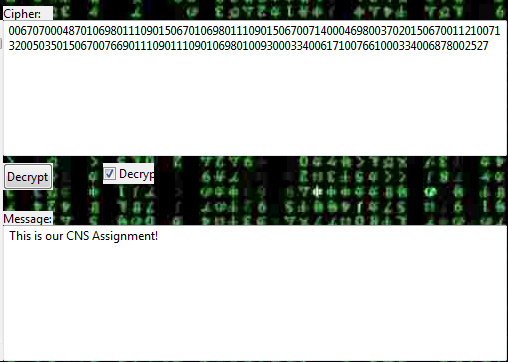
\includegraphics[scale=1]{proj.png}\\[1cm]    

% Title
\HRule \\[0.4cm]
{  \huge\bfseries Soft Set Theory for Soft Computing }\\[0.4cm]

\HRule \\[1cm]

% Author and supervisor
\begin{minipage}{0.8\textwidth}
\begin{flushleft} \large
\emph{By:}\\
Samir \textsc{Sheriff} [1RV09CS093]\\
Satvik \textsc{N} [1RV09CS095]\\


\end{flushleft}
\end{minipage}
\vfill

% Bottom of the page
{\large}

\end{center}

\end{titlepage}



\maketitle
\setcounter{secnumdepth}{1}

\section{Introduction}
Molodtsov initiated the concept of soft set as a new mathematical tool for dealing with uncertainties. Most of our traditional tools for formal modeling, reasoning and computing are crisp, deterministic and precise in character. However, there are many complicated problems in economics,
engineering, environment, social science, medical science etc.
that involve uncertainties. The Theory of Probability, Theory of
Fuzzy Sets,Theory of Intuitionistic Fuzzy Sets,Theory of Vague
Sets, Theory of Interval Mathematics and Theory of Rough Sets
are considered as mathematical tools for dealing with
uncertainties.

In 1999, Molodstov pointed out that these
theories which are considered as mathematical tools for dealing
with uncertainties, have certain limitations. He further pointed
out that the reason for these limitations is, possibly, the
inadequacy of the parameterization tool of the theory. The Soft
Set Theory introduced by Molodstov is quite different from
these theories in this context. The absence of any restrictions on
the approximate description in Soft Set Theory makes this
theory very convenient and easily applicable. Fuzzy set theory
proposed by Professor L. A. Zadeh in 1965 is considered as a
special case of the soft sets.

Current and soft mathematics can
co-exist and can be used consistently to solve real
world problems.




\section{Definitions}

\subsection{Structured Subsets}
According to the authors of this oh so marvelous paper, ideal membership functions for real world fuzzy sets are made from elastic material, because fuzzy sets should be able to tolerate certain
amount of perturbation or stretching. Mathematically, each perturbation is a new function, that consists of a set of functions,
each of which can be continuously stretched into
another function. Such a set of functions is a highly
structured subset of membership function space. 

\subsection{Soft Sets}
A fuzzy set, which is also called, in different parts of the world, a soft set, is an \textit{“abstract structured set”} of
membership function space. Such a structured subset
may be an equivalence class, a neighborhood, or
fuzzified structures in the membership function space. Soft sets are intended to capture and to defuse the conflicts among existing fuzzy theories. So a fuzzy set could be defined by 
\begin{enumerate}
\item{A collection of membership functions}
\item{that should be able to transform among themselves}
\end{enumerate}


\subsection{Neighbourhood Systems}
It is an abstraction of “near” or “negligible distances” in
geometry. A neighborhood system is an association that
assigns each datum a list of data that may or may not
contain the datum. It is natural and implementable, and used for  approximate retrieval in databases and approximate reasoning in knowledge bases

The central notion here is neighborhood systems. It
is an abstraction of “near” or “negligible distances” in
geometry. A neighborhood system is an association that
assigns each datum a list of data that may or may not
contain the datum. It is natural and implementable. So current and soft mathematics can
co-exist and can be used consistently to solve real
world problems.

Neighborhood systems express the semantics of
nearby spaces. Let p be an object (or datum) in the universe or
space X. 

\begin{itemize}
\item{A neighborhood, denoted by N(p), or simply N,
of p is a non-empty subset of X, which may or
may not contain the object p.}
\item{Any subset that contains a
neighborhood is a neighborhood.}
\item{A neighborhood
system of object p, denoted by NS(p), is a non-empty
maximal family of neighborhoods of p.}
\item{A neighborhood system of X, denoted by NS(X) is the
collection of NS (p) for all objects p in X.}
\item{If a
neighborhood system NS(X) that satisfies certain
axioms, then X is a topological space. In
general, X is a Frechet (V) space.}
\item{From this view, rough set theory is a special case of the
neighborhood system theory.}
\end{itemize}


\subsection{Soft sets, defined using Neighbourhood Systems}
A real world fuzzy set is defined abstractly by a neighborhood systems of membership function space. Neighborhood systems translate the real world problem into a mathematical problem. So our ultimate goal is to axiomatize fuzzy sets through such neighborhood
systems.


\subsection{Membership Function Space}
Let U be the universe of discourse, and let
FX : U \begin{math} \rightarrow \end{math} M
be a map, where M is, in general, a membership space. 

FX is called a membership function; FX(x) is called the grade or degree of membership of x \begin{math} \in \end{math} U. 

If M is the set of two elements $\{$0, 1$\}$, then FX is the
characteristic function of a classical crispy set. If M is a
unit interval [0, 1], then FX is the membership function of a
classical fuzzy set.

Let be a collection of fuzzy sets on U. Each fuzzy set is defined by a neighborhood (may be a singleton) in the membership function space;







The developments of various generalized set theories form a
beginning of a "soft mathematics” and may provide a
foundation for soft computing. This paper is one of our
attempt to provide a solid set theory for soft computing.


\subsection{How Public-key Cryptosystems Work}
The distinguishing technique used in public-key cryptography is the use of asymmetric key algorithms, where the key used to encrypt a message is not the same as the key used to decrypt it. Each user has a pair of cryptographic keys - a public encryption key and a private decryption key. The publicly available encrypting-key is distributed, while the private decrypting-key is kept secret. Messages are encrypted with the recipient's public key, and can be decrypted only with the corresponding private key. The keys are related mathematically, but the parameters are chosen so that determining the private key from the public key is either impossible or prohibitively expensive. 


\subsection{Schmidt-Samoa Public-key Cryptosystem}
The Schmidt-Samoa cryptosystem is an asymmetric cryptographic technique, whose security, like Rabin and RSA depends on the difficulty of integer factorization.
\begin{itemize}
\item{Key generation}
\begin{itemize}
\item{}Choose two large distinct primes p and q and compute $N = p^2 \times q$
\item{}Compute $d = N-1$ mod $lcm(p - 1, q - 1)$
\item{}Now N is the public key and d is the private key.
 \end{itemize}


\item{\textbf{Encryption}} - 
To encrypt a message m we compute the cipher text as $c = m^N mod N$
 
\item{\textbf{Decryption}}
To decrypt a cipher text c we compute the plaintext as $m = c^d mod (p\times q)$ which like for Rabin and RSA can be computed with the Chinese remainder theorem.



\item{\textbf{Security}} - 
The algorithm, like Rabin, is based on the difficulty of factoring the modulus N, which is a distinct advantage over RSA. That is, it can be shown that if there exists an algorithm that can decrypt arbitrary messages, then this algorithm can be used to factor N.
\end{itemize}

\section{Previous Cryptosystems}
\subsection{RSA Cryptosystem}
RSA stands for Ron Rivest, Adi Shamir and Leonard Adleman, who first publicly described it in 1977.

\begin{itemize}
\item{\textbf{Key Generation}}
\begin{itemize}
\item{}Let N = $p\times q$ be a product of two prime numbers
\item{}Compute $\varphi(n) = (p – 1)(q – 1)$, where $\varphi$ is Euler's totient function.
\item{}Choose an integer e such that $1 \leq e \leq \varphi(n)$ and greatest common divisor of (e, $\varphi(n)$) = 1; i.e., e and $\varphi(n)$ are co-prime.
\item{}Determine d as: d = $e^{-1}$ (mod $\varphi(n)$), d is the multiplicative inverse of e mod $\varphi(n)$.
 \end{itemize}

\item{\textbf{Encryption}}:    Let M be a message, and c the ciphertext. Then,
        	$c = m^e (mod n)$
\item{\textbf{Decryption}}:  $m = c^d (mod n)$
By construction, $d^e= 1$ mod $\varphi(n)$. The public key consists of the modulus n and the public (or encryption) exponent e. The private key consists of the modulus n and the private (or decryption) exponent d which must be kept secret.
\end{itemize}
\subsection{Rabin\'s Cryptosystem}
In 1979, Michael Rabin suggested a variant of RSA with public-key exponent 2, which he showed to be as secure as factoring.
\begin{itemize}
\item{\textbf{Key Generation}}
\begin{itemize}
\item{}Choose two large distinct primes p and q.
\item{}Let n=pq. Then n is the public key. The primes p and q are the private key
 \end{itemize}

\item{\textbf{Encryption}}:  For the encryption, only the public key n is used. The process follows -
Let  P = \{0,...,n-1\} be the plaintext space (consisting of numbers) and $m \in P$ be the plaintext. Now the ciphertext  is determined by $c = m^2 $(mod n).


c is the quadratic remainder of the square of the plaintext, modulo the key-number n.
\item{\textbf{Decryption}}:
To decode the ciphertext, the private keys are necessary. The process follows:
If c and r are known, the plaintext is then $m \in \{0,$...,$n-1$\} with $m^2=c$ (mod r). For a composite r (that is, like the Rabin algorithm's ) there is no efficient method known for the finding of m. If, however r is prime (as are p and q in the Rabin algorithm), the Chinese remainder theorem can be applied to solve for m.

Thus the square roots
$ m_p = \sqrt{c}$ mod p
and
$ m_q = \sqrt{c}$ mod q must be calculated
\end{itemize}


\section{Implementation}
\lstinputlisting[language=Java]{Schmidt_Samoa_Encryptor.java}
%\begin{figure}[h!]
%  \centering
%   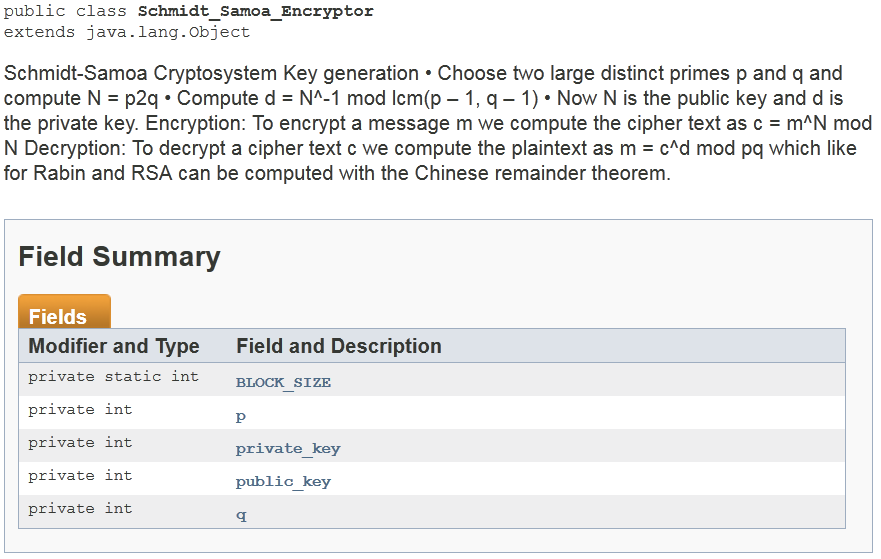
\includegraphics[scale=1.0]{schmidt_field.png}
%  \caption{Experimental Results}
%\end{figure}
%
%\begin{figure}[h!]
%  \centering
%   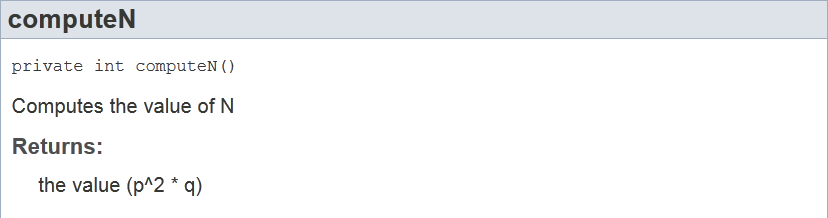
\includegraphics[scale=1.0]{computeN.png}
%  \caption{Experimental Results}
%\end{figure}
%
%\begin{figure}[h!]
%  \centering
%   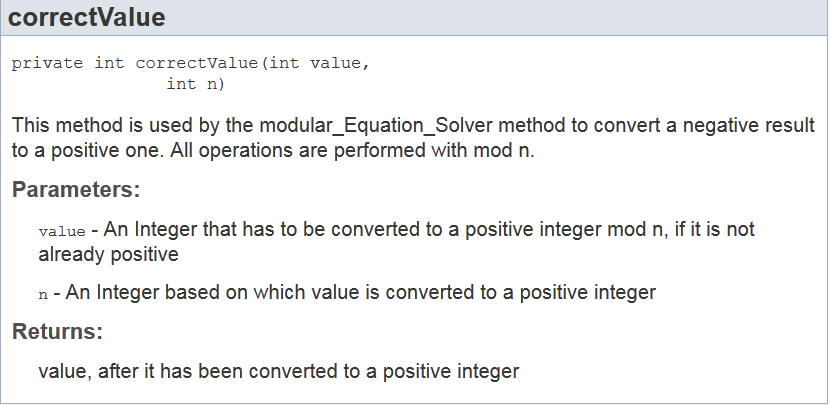
\includegraphics[scale=1.0]{correctValue.png}
%  \caption{Experimental Results}
%\end{figure}



%\begin{figure}[h!]
%  \centering
%   \includegraphics[scale=0.50]{watlas.png}
%  \caption{A small portion of the Watershed Atlas for British Columbia that was
%developed using an IBM Informix ORDBMS.}
%\end{figure}


\begin{thebibliography}{9}
\bibitem{pap}
Katja Schmidt-Samoa, 
\emph{A New Rabin-type Trapdoor Permutation Equivalent to Factoring and Its Applications}. TechnischeUniversit. samoa@informatik.tu-darmstadt.de

\bibitem{wiki}
  Schmidt-Samoa Cryptosystem - 
 \url{http://en.wikipedia.org/wiki/Schmidt-Samoa_cryptosystem}
\bibitem{textbook}
 Rivest, R.; A. Shamir; L. Adleman (1978). \emph{"A Method for Obtaining Digital Signatures and Public-Key Cryptosystems"}. Communications of the ACM 21 (2): 120–126. doi:10.1145/359340.359342

\bibitem{pdp} Joe Hurd, Blum Integers (1997) -  \url{http://www.gilith.com/research/talks/cambridge1997.pdf}
\bibitem{pap}Rabin, Michael. \emph{Digitalized Signatures and Public-Key Functions as Intractable as Factorization}. MIT Laboratory for Computer Science, January 1979.

\bibitem{link}Katja Schmidt-Samoa - \emph{Contributions to Provable Security and Efficient Cryptography}.\\\url{http://tuprints.ulb.tu-darmstadt.de/708/1/Diss.Schmidt-Samoa.pdf}
\end{thebibliography}
\newpage
\section{Screenshots}
\begin{figure}[h!]
  \centering
   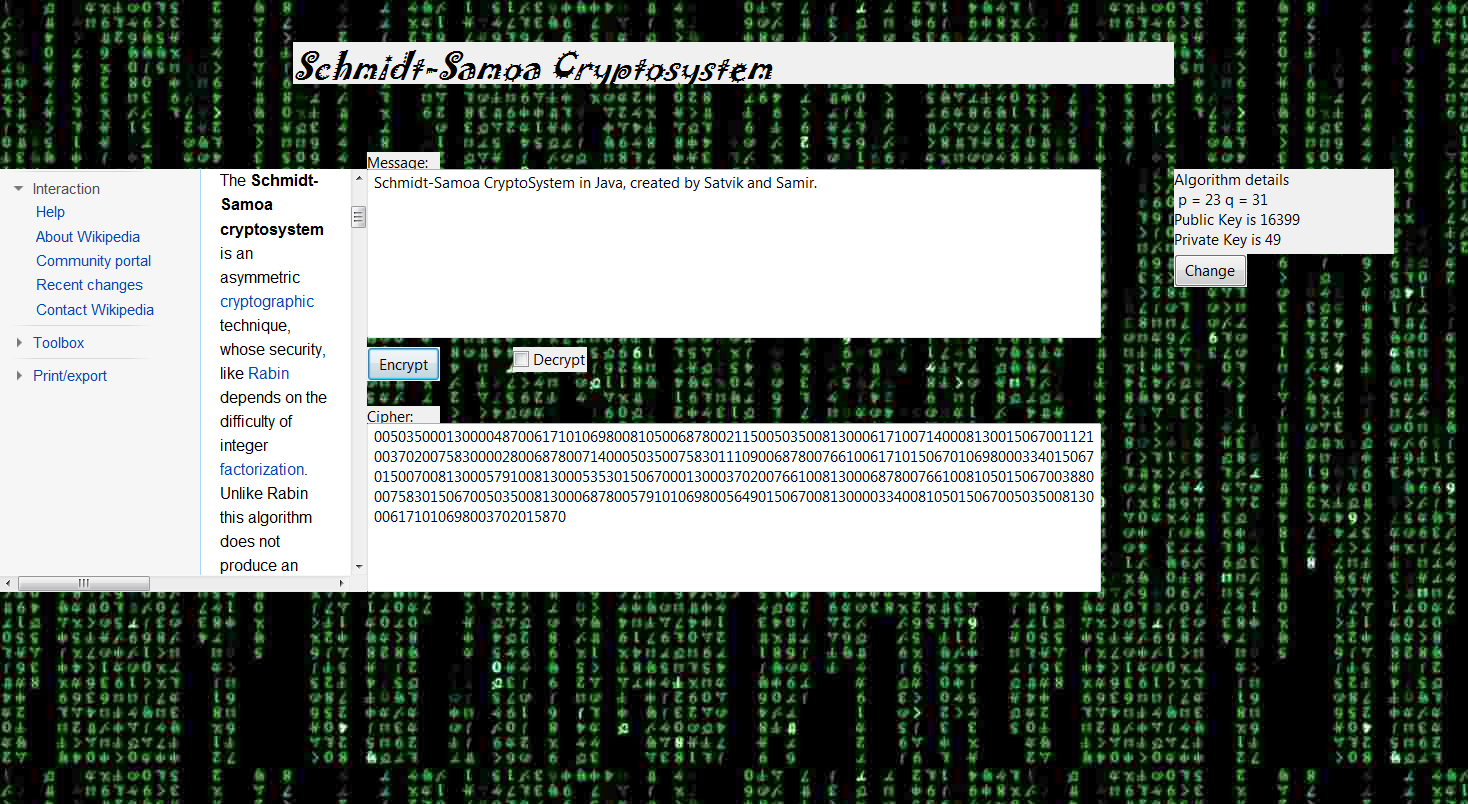
\includegraphics[scale=0.50]{encrypt.png}
  \caption{Encryption using the Schmidt-Samoa algorithm}
\end{figure}

\begin{figure}[h!]
  \centering
   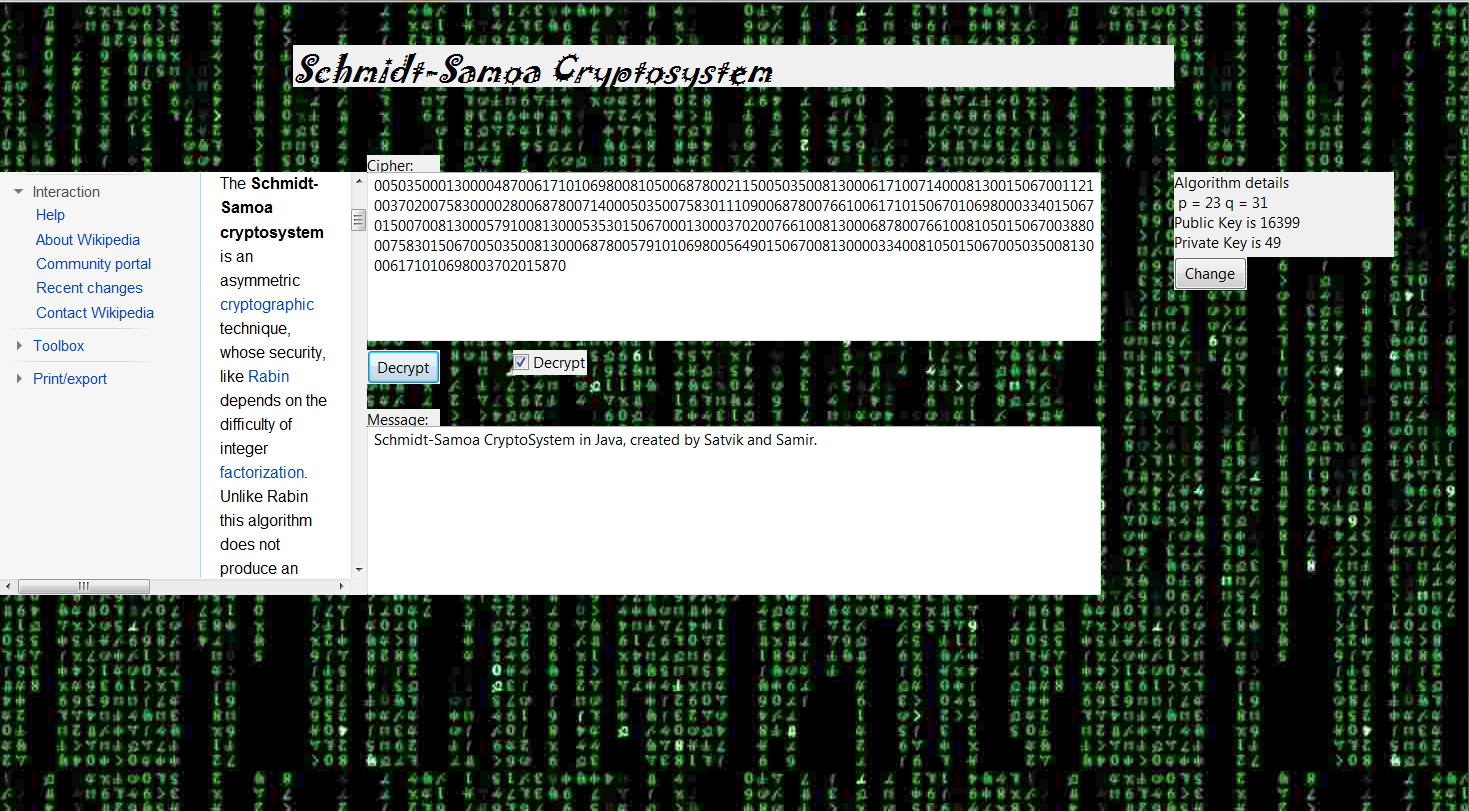
\includegraphics[scale=0.50]{decrypt.png}
  \caption{Decryption using the Schmidt-Samoa algorithm.}
\end{figure}


\end{document}
